\section{Performance Evaluation}\label{evaluation}
To evaluate our algorithms,
we use the real  network 
CERNET2 (14 nodes, 16 links), Abilene (11 nodes, 14 links), NJLATA (11 nodes, 23 links), TORONTO (25 nodes, 55 links) and
USLD (28 nodes, 45 links)
and five ISP topologies which are measured by Rocketfuel\cite{2004148100061},
including   AS1221 (108 nodes, 153 links),
AS1239 (315 nodes, 972 links), 
AS1755 (87 nodes, 161 links), AS3257 (161 nodes, 328 links), 
AS3967 (79 nodes, 147 links), and AS6461  (128 nodes, 372 links) .
We also generate synthetic topologies with BRITE \cite{medina2001brite},
using parameters as listed in Table \ref{britetable}.
%In this section, we first show how link failures are modeled in our evaluation.
For similarity, we use a simple model to characterize link failure events.
The fail probability of each link $e$
is randomly generated in the range from 0 to 0.0001.
All the simulations are conducted on a PC with Intel
i5 CPU, 1.7GHz and 1.5G Memory.
Because neither DMPA nor TBFH can implement the NPC rule, IAC can only implement DC rule, so in the experiment we only compare the performance of
the three methods on achieving  DC rule. %Because IAC and IAC-NA have similar performance in realizing DC rule, IAC/IAC-NA is used to represent these two algorithms in the following section.
%In the following section, we will use IAC/IAC-NA to denote the IAC and IAC-NA.
\begin{table}[h]
%% increase table row spacing, adjust to taste
\normalsize
\renewcommand{\arraystretch}{1}
\caption{Parameters for BRITE}
\label{britetable}
\begin{center}
\begin{tabular}{c|c|c|c}
\hline
Model& N &   HS & LS  \\
\hline
Waxman & 20-1000&1000&100\\
\hline
\hline
m&NodePlacement &GrowthTypem & ${alpha}$  \\
\hline
2-40 & Random&Incremental&0.5\\
\hline
\hline
 ${beta}$ & BWDist &BwMin &BwMax \\
 \hline
0.5&Heavy Tail&100.0&1024.0\\
\hline
\end{tabular}
\end{center}
\end{table}
\subsection{Computation complexity}
Theoretical analysis has indicated that the time complexity of IAC/IAC-NA is less than that of building of a shortest path tree, which has a great advantage over DC, TBFH and DMPA. In order to further verify the computational performance, we make simulations on different topologies. In this section, we evaluate the computational overhead of different algorithms. In order to avoid the uncertain factors impact the algorithm��s performance. The computational overhead of an algorithm is defined as the ratio of computation time of the algorithm to that of SPF (shortest path first).
\begin{figure}[t]
\centering
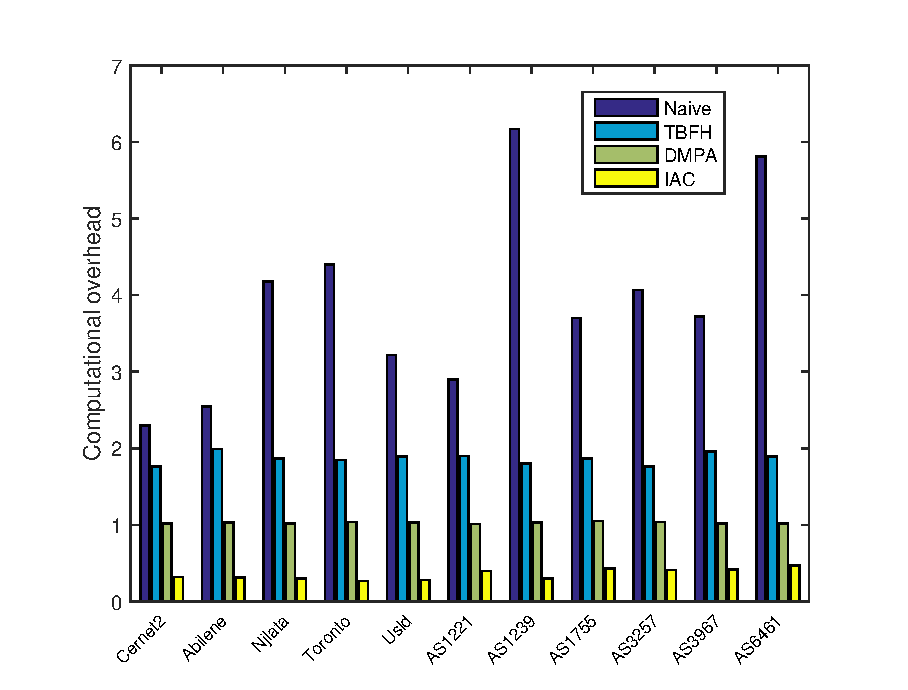
\includegraphics[width=3in]{realcomputationoverhead}
%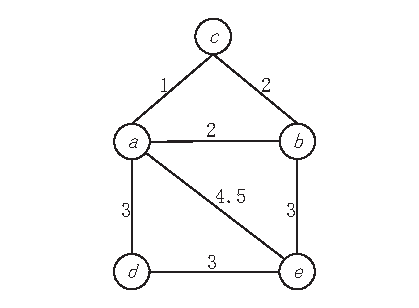
\includegraphics[width=3in]{lfaexample}
\caption{Computation overhead on real topologies}
\label{realtopologytime}
\end{figure}
\begin{figure}[t]
\centering
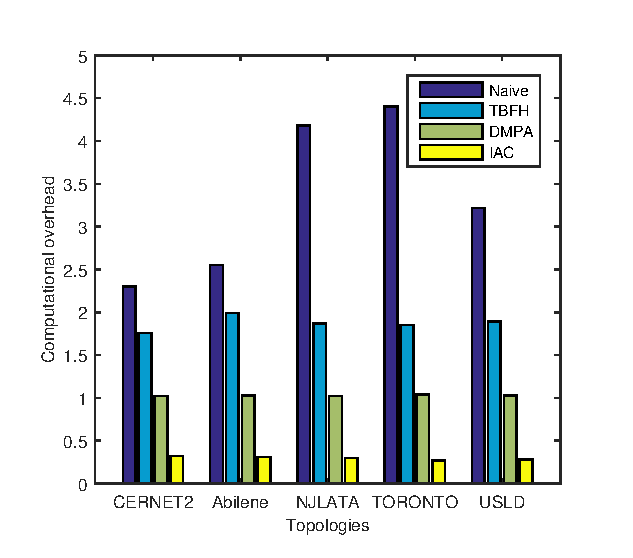
\includegraphics[width=3in]{rocketcomputationoverhead}
%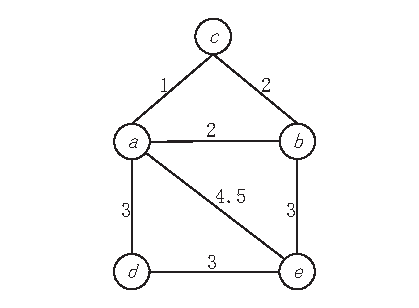
\includegraphics[width=3in]{lfaexample}
\caption{Computation overhead on  measured topologies}
\label{rockettopologytime}
\end{figure}
Fig. \ref{realtopologytime} and Fig. \ref{rockettopologytime} respectively indicate the computational overhead obtained by different algorithms on real and Rocketfuel topologies. From the Fig. \ref{realtopologytime} and Fig. \ref{rockettopologytime}, we can see that IAC/IAC-NA has the lowest computation overhead among all the algorithms. The computation overhead of IAC/IAC-NA is less than computing a SPT, while DMPA need to construct a SPT and TBFH need to compute two SPTs. The computation overhead of DC is proportionally to the degree of the network average node degree.
\begin{figure}[t]
\centering
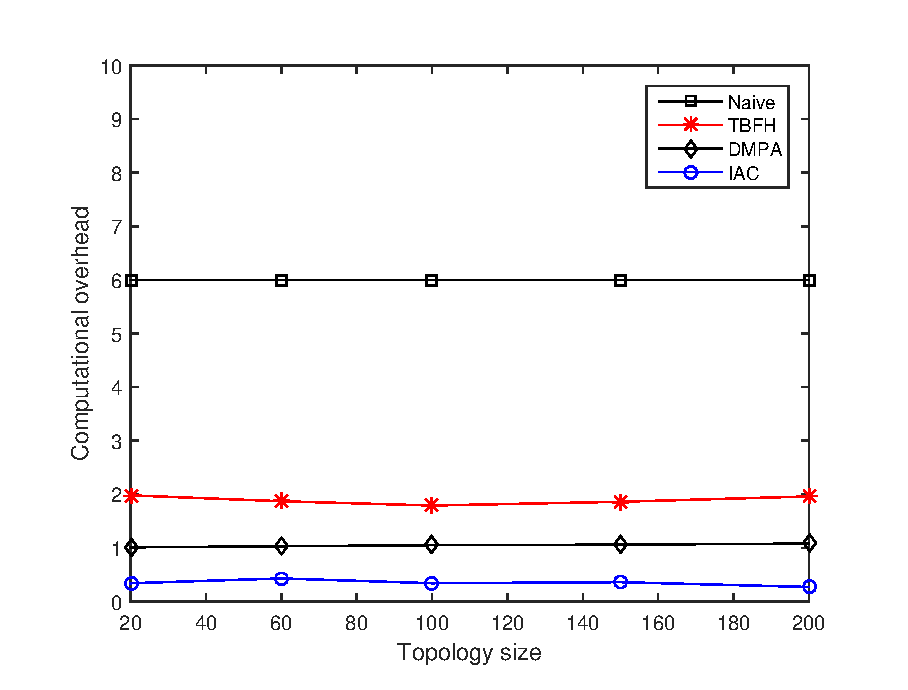
\includegraphics[width=3in]{tscomputationoverhead}
\caption{Computation overhead on generated topologies when average node degree is 6}
\label{topologysize200}
\end{figure}
\begin{figure}[t]
\centering
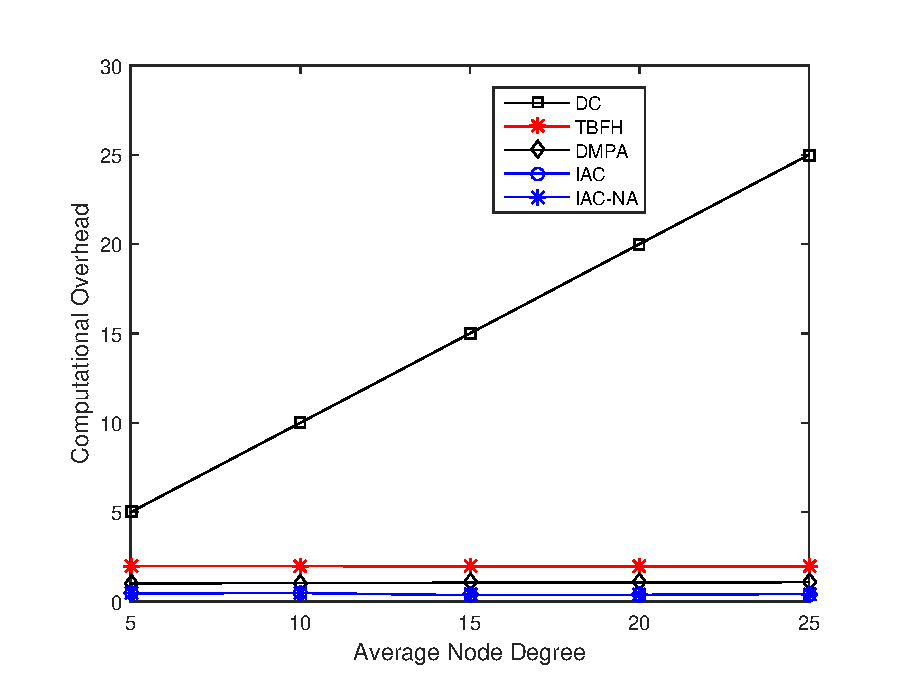
\includegraphics[width=3in]{degcomputationoverhead}
\caption{Computation overhead on generated topologies when topology size is 200}
\label{nodedegree6}
\end{figure}
\begin{figure}[t]
\centering
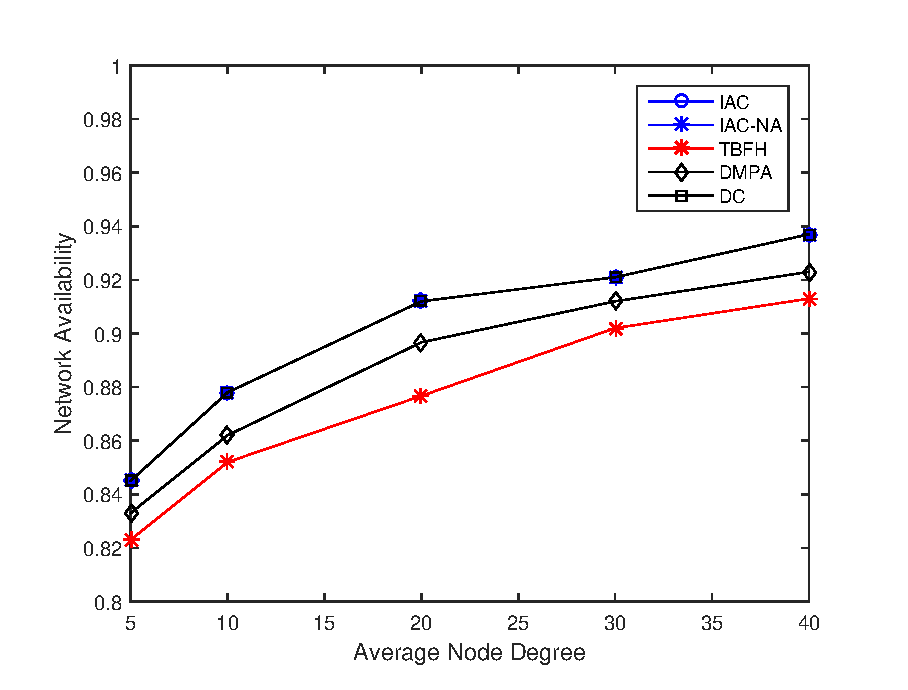
\includegraphics[width=3in]{nodedegree}
\caption{Network Availability on Generated Topologies When Topology Size=200}
\label{avdeg}
\end{figure}
\iffalse
\begin{figure*}[t]
        \centering
        \begin{subfigure}[b]{0.32\textwidth}
                \centering
                \includegraphics{abilenedeploy}
                \caption{$T_{c}$}
              \label{spttree}
        \end{subfigure}
        \begin{subfigure}[b]{0.32\textwidth}
                \centering
                \includegraphics{exodusdeploy}
                \caption{$T'_{c}$ when $L(c,a)=0$}
                \label{spttreechange1}
        \end{subfigure}
         \begin{subfigure}[b]{0.32\textwidth}
                \centering
                \includegraphics{sprintdeploy}
                \caption{$T'_{c}$ when $L(c,b)=0$}
                \label{spttreechange2}
        \end{subfigure}
        \caption{An example for explaining some Theorems}
        \label{theoremexample}
\end{figure*}
\fi
\iffalse
\begin{figure}[t]
\centering
\includegraphics[width=3in]{abilenedeploy}
\caption{Incremental Deployment on Abilene}
\label{abilene}
\end{figure}

\begin{figure}[t]
\centering
\includegraphics[width=3in]{exodusdeploy}
\caption{Incremental Deployment on Exodus}
\label{exodus}
\end{figure}

\begin{figure}[t]
\centering
\includegraphics[width=3in]{sprintdeploy}
\caption{Incremental Deployment on Sprint}
\label{sprint}
\end{figure}

\begin{figure}[t]
\centering
\includegraphics[width=3in]{top1000}
\caption{Incremental Deployment on Generated Topologies When Topology Size=1000}
\label{top100avi}
\end{figure}
\fi
\iffalse
\begin{figure}[t]
\centering
\includegraphics[width=3in]{topodeploy200}
\caption{Incremental Deployment on Topology=200}
\label{abilene}
\end{figure}

\begin{figure}[t]
\centering
\includegraphics[width=3in]{topodeploy500}
\caption{Incremental Deployment on Topology=500}
\label{exodus}
\end{figure}

\begin{figure}[t]
\centering
\includegraphics[width=3in]{topodeploy1000}
\caption{Incremental Deployment on Topology=1000}
\label{sprint}
\end{figure}
\fi
Fig. \ref{topologysize200} illustrates the relationship between the computation overhead and topology size on generated topologies when the average node degree is 6. As Fig. \ref{topologysize200} shows, the computation overhead of all the algorithms does not depend on the topology size. The computation overhead of IAC/IAC-NA is lowest among all the algorithms.

Fig. \ref{nodedegree6} presents the relationship between the computation overhead and average node degree on generated topologies when the topology size is 200.
As the average node degree increases, the computation overhead of DC increases accordingly. And also IAC/IAC-NA has the highest performance among all the algorithms. Therefore, the above experiment results are consistent with the theoretical analysis described above.
\iffalse
 \begin{table}[h]
\centering
\renewcommand{\arraystretch}{1}
\caption{Computation time for Real Topologies}
\label{comparison}
\begin{tabular}{c|c|c|c|c|c|c}
\hline
&\multirow{2}{*}{Network}& \multicolumn{5}{|c}{Computation time ($\upmu$s)} \\
\cline{3-7}
& & OSPF &LFC & TBFH & MNP&MNP-e\\
\hline
Real& Abilene& 6.82&7.27 & 6.97 & 6.83&6.52\\
\hline
\multirow{3}{*}{Measured}& Exodus & 44.36 &128.29&88.76&50.23 &42.34\\
\cline{2-7}
& Telstra & 49.45 &163.43&100.34&54.34&46.23 \\
\cline{2-7}
& Tiscali & 79.45 &398.34&183.56&83.45 &75.34\\
\cline{2-7}
& Sprint &  140.23&906.78 &368.12 & 150.12 &137.34\\
\hline

\end{tabular}
\end{table}
\fi
\subsection{Protection ratio and The average number of next hops}
In this section, we will use the protection ratio  and the average number of next hops to measure the path diversity of different algorithms.
The protection ratio is defined as
\begin{equation}
Pr=\frac{\sum\limits_{c,d\in V, c\neq d}{K(c,d)}}{|V|*(|V|-1)}
\end{equation}
\begin{equation}
K(c,d)=\begin{cases}
1&\mbox{$|N_c(d)|\geq 2$}\\
0&\mbox{$|N_c(d)|=1$}
\end{cases}
\end{equation}
The average number of next hops
describes the number of opportunities packets can be deflected off the
shortest path.
For both of the above two metrics, larger is better. 

Fig. \ref{prreal} and Fig. \ref{prrocket} respectively depict the protection ratio obtained by different algorithms on real and measured topologies.
Fig. \ref{prd} presents the relationship between the protection ratio and average node degree on generated topologies
when the topology size is 200.
Fig .\ref{number} depicts  the average number of next hops obtained by different algorithms on real and Rocketfuel topologies.
Fig .\ref{abicumulative} and  Fig .\ref{cercumulative} show
the cumulative distribution of the average number of next hops for Abilene, and CERNET2.
\begin{figure}[t]
\centering
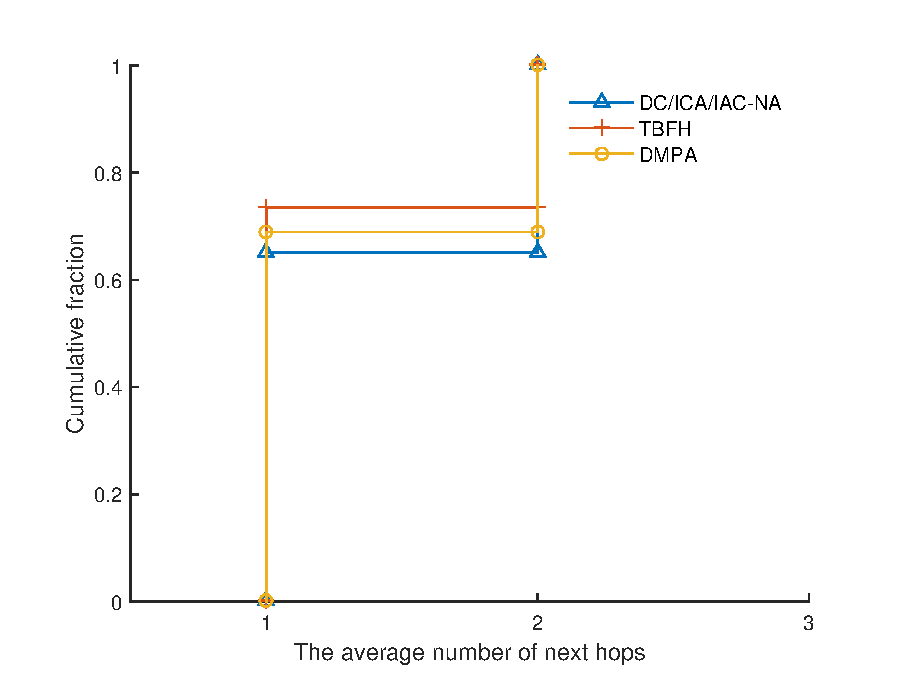
\includegraphics[width=3in]{Abilenecumulative}
\caption{Cumulative distribution distribution of the average number of next hops on Abilene topology}
\label{abicumulative}
\end{figure}
\begin{figure}[t]
\centering
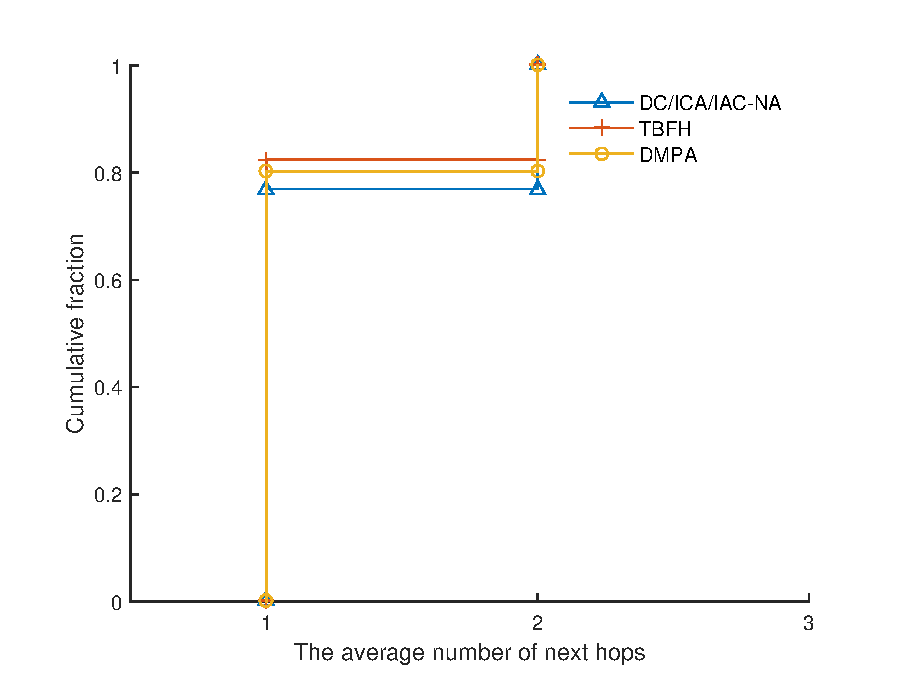
\includegraphics[width=3in]{CERNET2cumulative}
\caption{Cumulative distribution distribution of the average number of next hops on CERNET2 topology}
\label{cercumulative}
\end{figure}
We made several conclusions. First, IAC/IAC-NA and DC are more
flexible than TBFH and DMPA. They have more deflection choices in all
the experiment networks. Second, the
larger networks can provide more opportunities to detour.
\iffalse 
Last,
For IAC/IAC-NA and DC, more than
40\% of routers have more than one next hop in all simulated topologies.
and this advantage is more pronounced in large topologies.
From Fig. \ref{prreal}, Fig. \ref{prrocket} and Fig. \ref{prd}, we can see that INC, INC-NA and DC have the similar protection ratio, which have better performance than both of DMPA and TBFH.
\fi

Since both of the above two metrics cannot accurately describe end-to-end network availability. Therefore, we will use network availability to measure the end-to-end availability of different algorithms in the next section.
\begin{figure}[t]
\centering
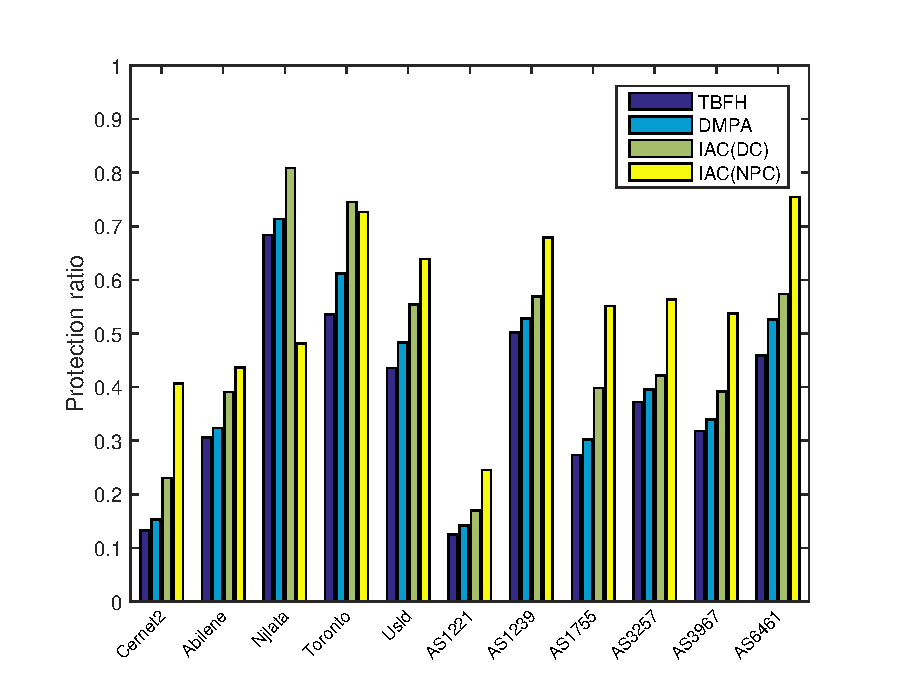
\includegraphics[width=3in]{protectionratioreal}
\caption{Protection ratio on real topologies}
\label{prreal}
\end{figure}
\begin{figure}[t]
\centering
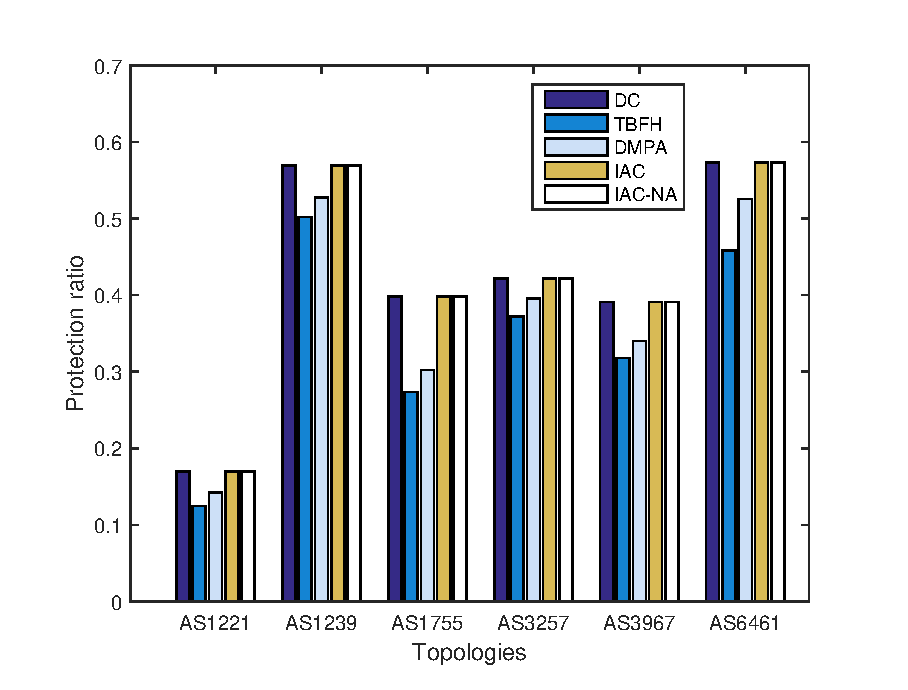
\includegraphics[width=3in]{protectionratiorocket}
\caption{Protection ratio on measured topologies}
\label{prrocket}
\end{figure}
\begin{figure}[t]
\centering
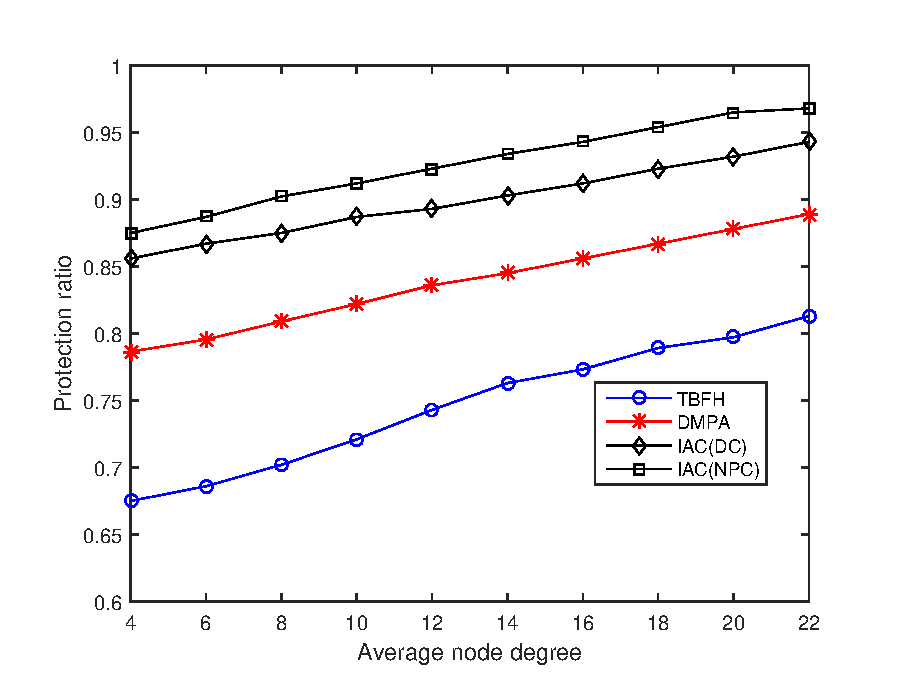
\includegraphics[width=3in]{protectionratiodegree}
\caption{Protection ratio on generated topologies when topology size is 200}
\label{prd}
\end{figure}
 \subsection{Network availability}
 We formally define the network availability $A(G)$ as follows (similar to that in \cite{ReliabilityAnalysis}),
and use it as a main metric to evaluate the protection capability of different schemes.

The end-to-end availability of a source-destination ($s$-$d$) pair is defined as the
probability that the packets can be correctly forwarded from $s$ to $d$.
Assume that there exist $n$ different forwarding paths from $s$ to $d$,
the $i$-th which is denoted by $p_{i}(s,d)$.
We also use $P_{i}(s,d)$ to represent the set of links on the $p_{i}(s,d)$.
Further, let the event that $p_{i}(s,d)$ works be denoted by $A_{i}(s,d)$,
whose probability can be expressed as:
\begin{equation}\label{ir}
P(A_{i})=\prod\limits_{\forall (m,n) \in P_{i}(s,d)}{r(m,n)}
\end{equation}


According to the Inclusion-Exclusion principle \cite{feller},
the end-to-end availability of a source-destination pair can be expressed as:

\begin{equation}\label{asd}
A(s,d)=\sum\limits_{k=1}^{n}{(-1)^{(k-1)}S_k}
\end{equation}
where $S_k$ denote the sum of the probabilities that a unique set of $k$ paths
from $s$ to $d$ are simultaneously working, which is further expressed as:

\begin{eqnarray}\label{sk}
S_{k}&=&\sum\limits_{i<j< \cdots <k}{P(A_{i} \cap A_{j}\cdots \cap A_{k})} \nonumber \\
&=&\sum\limits_{i<j< \cdots <k} \left(\prod\limits_{ (m,n) \in P_{i}(s,d) \cup P_{j}(s,d) \cup \dots \cup P_{k}(s,d)}{r(m,n)}\right) \nonumber
\end{eqnarray}


Then, the network availability can be computed as

\begin{equation}
A(G)=\frac{\sum\limits_{s,d \in V, s \neq d}{A(s,d)}}{|V|*(|V|-1|)}
\end{equation}
\begin{table}[t]
\centering
%\normalsize
\footnotesize
%\small
%\renewcommand{\arraystretch}{1}
\caption{Network Availability for Real and Measured Topologies}
\label{Availability}
\begin{tabular}{c|c|c|c|c|c}
\hline
&\multirow{2}{*}{Network}& \multicolumn{4}{|c}{Network Availability($\%$)} \\
\cline{3-6}
& & IAC/IAC-NA &DC & TBFH &  DMPA\\
\hline
\multirow{5}{*}{Real}
& CERNET2& 99.93&99.93 &97.37& 98.54 \\
\cline{2-6}
& Abilene& 99.97&99.97 &97.34& 98.63\\
\cline{2-6}
& NJLATA& 99.93&99.93 &96.87& 97.81 \\
\cline{2-6}
& TORONTO& 99.87&99.87 &97.65& 98.74 \\
\cline{2-6}
& USLD& 99.94&99.94 &97.34& 98.57 \\
\cline{2-6}
\hline
\multirow{5}{*}{Measured}
& AS1221 & 99.94 &99.94&96.35&97.25 \\
\cline{2-6}
& AS1239 &  99.96&99.96 &95.67&96.37 \\
\cline{2-6}
& AS1755 &  99.98&99.98&97.38&98.29 \\
\cline{2-6}
& AS3257 & 99.91&99.91&95.48&96.35 \\
\cline{2-6}
& AS3967 & 99.94 &99.94&95.78&96.89 \\
\cline{2-6}
& AS6461 & 99.96 &99.96&95.82&97.03 \\
\cline{2-6}

\hline
\end{tabular}
\end{table}

Table \ref{Availability} provides the network availability provided by each protection scheme, on the real and measured topologies. From the results, we can see that IAC/IAC-NA has a clear advantage over TBFH and DMPA, and has the same performance as DC.

Fig. \ref{avdeg} illustrates the relationship between the network availability and the average node degree.
As Fig. \ref{avdeg} shows, as the average node degree increase, the network availability increases too. Note that when the average node degree increases, all schemes provide better protection results, while IAC/IAC-NA and DC are always much better than DMPA and TBFH.
\iffalse
\subsection{Incremental Deployment}
In this paper, we have proposed IAC/IAC-NA,
which is compatible with nowadays link-state routing
protocol, such as OSPF and IS-IS.
ISPs can deploy the algorithm in two ways, full deployment and incremental deployment.
However, full deployment is a burden for all ISPs.
Therefore, incremental deployment is employed in practice.
In this section, we will address the incremental deployment problem.
A node-by-node incremental deployment scheme is highly preferred.
The optimal deployment can be defined as:\\
\textbf{Optimal Deployment:}
Given a graph $G(V,E)$ and a positive integer $k$, our objective is to find a deployment $M$ where, $M \subset V$ and $|M|$=$k$ such that network availability is maximized.
\iffalse
\begin{algorithm}[h]
\caption{GreedyDeploy($G, m$)}
\label{deployment1}
\begin{algorithmic}[1]
\STATE $M\leftarrow \emptyset$
\WHILE {$|M|\leq k$}
\STATE $a\leftarrow max(B(a,M))$
\STATE $M\leftarrow M\cup \{a\}$
\ENDWHILE
\RETURN $S$
\end{algorithmic}
\end{algorithm}
\fi

We first define a benefit function for a node with respect to
the nodes which have been deployed.
Let $a$ be an arbitrary node in the network.
The benefit of node $a$ with respect to $M$, which is the nodes have been already deployed, is
denoted by $B(a,M)$, which can be expressed as:
\begin{equation}\label{benefit}
B(a,M)=A(G,M\cup \{a\})-A(G,M)
\end{equation}

It has been proved in \cite{zhang2013rpfp} that
finding the optimal deployment is NP-Complete.
Because the Optimal Deployment is NP-Complete problem.
With regard to the large $k$ and large topologies, a straight-forward
exhaustive search is computationally unacceptable.

\iffalse
A  simple greedy heuristic algorithm (GreedyDeploy)
 for selecting nodes to be deployed. The inputs of algorithm  is $k$.
The outputs of the algorithm  is the optimal deployment $M$.
The algorithm  goes through several iterations,
in each iteration, we will select a node which  has the maximum benefit to be deployed.
\fi

\iffalse
We propose an improved algorithm (SimulateDeploy) roughly modeled
after the Simulated Annealing probabilistic metaheuristic \cite{retvari2011optimizing}.
The main idea is that we first randomly select the deployed nodes set $M$.
Then finding the best $S'$
and accept it if either $S'$ can obtain lager network availability
than $S$ or  the temperature $T$ of the system is sufficiently large.
As the algorithm progresses we gradually
reduce $T$, thus the system will increasingly tend to get stuck
 in a local optimal solution.


We develop  Algorithm \ref{deployment} to solve the Optimal Deployment issue.
First, we randomly select a set of $M$, $M \subset V$ and $|M|$=$k$ , and set an initial system temperature (lines 1-2).
Let tuple $(c,c')$ be a pair of nodes such that  $c \in M$  and  $c' \notin M$,
we unconditionally accept this $c'$ either if it is
better than the previous one or if a random number generated temperature is less than $T$ (lines 4-5).
This can guarantee the algorithm escape from a local minimum.
\fi
\begin{algorithm}[h]
\caption{SimulateDeploy}
\label{deployment}
\begin{algorithmic}[1]
\STATE $T\leftarrow T_0 $
\STATE generate the initial set $M$ randomly
\REPEAT
%\STATE $\forall c \in M  and  c' \notin M$
\IF {$A(G,(M-c) \cup c')>A(G,M)\wedge T>random(T_0)$ }
\STATE $M\leftarrow (M-c) \cup c'$
\ELSE
\STATE $T\leftarrow T-1$
\ENDIF
\UNTIL{$T>T_{0}\land$ no such $(c,c')$ exists}
\RETURN $M$
\end{algorithmic}
\end{algorithm}

We propose an improved approximate algorithm roughly modeled
after the Simulated Annealing probabilistic metaheuristic \cite{retvari2011optimizing}.
The main idea is that we first select $M$, which is the solution generated randomly.
Then finding the best solutions
and accept it if either they can obtain lager network availability
than the former one or  the temperature $T$ of the system is sufficiently large.
As the algorithm progresses we gradually
reduce $T$, thus the system will increasingly tend to get stuck
in a good quality local minimum.
We develop  Algorithm \ref{deployment} to solve the Optimal Deployment issue.
The inputs of Algorithm \ref{deployment} is $k$.
The outputs of the Algorithm \ref{deployment} is the optimal deployment $M$.
First, we generate a set of $M$ for $M \subset V$ and $|M|$=$k$ randomly, and set an initial system temperature (lines 1-2).
Let tuple $(c,c')$ be a pair of nodes such that  $c \in M$  and  $c' \notin M$,
we unconditionally accept this $c'$ either if it is
better than the previous one or if a random number generated temperature is less than $T$ (lines 4-5).


Our proposed algorithm is compatible with the currently deployment intra-domain routing protocol.
In this section, we will show the relationship between the number of deployed nodes and network availability. In our experiment, we implement Algorithm \ref{deployment} respectively on real and generated topologies.
We repeated ten experiments, the final value for each topology is the average of the results.

Fig. \ref{abilene}, Fig. \ref{exodus}  and Fig. \ref{sprint} depict the relationship between the number of deployed nodes and network availability in  real networks and measured  topologies,
while Fig. \ref{top100avi} shows  the relationship between the number of deployed nodes and network availability in generated topology when the topology size is 1000.
Note that, as the node deployed ratios increases, the network availability increase too, our proposed algorithm can provide comparable performance to that of DC. Through this experiment, we will give ISPs a recommendation that they
can give priority to the deployment of some key nodes, and finally the whole network deployment.
In the actual deployment, we can give priority to the deployment of key nodes.
%We can also see that when a deployment on only 40\% nodes already increase the network availability clearly.
\fi

